\section{Ulteriori strumenti}

Durante lo sviluppo del progetto è stato necessario sviluppare degli strumenti aggiuntivi che facilitassero il lavoro e completassero le funzionalità del marketplace. Nei prossimi paragrafi verranno analizzati questi strumenti.

\subsection{Creazione automatica NFTs}

Nella fase iniziale del progetto, prima dell'aggiunta della funzionalità di creazione di un NFT, è stato necessario creare manualmente gli NFTs per poterli visualizzare all'interno del marketplace. Essendo la creazione di un NFT completo di immagine e metadati un'operazione lunga e ripetitiva, è stato deciso di creare uno script che automatizzasse questo processo. Con lungimiranza nella possibile evoluzione del progetto, è stato deciso di creare uno script che permettesse di creare una collezione autogenerando le immagini e i metadati, nonché di pubblicarli su IPFS e blockchain.

Le immagini vengono generate utilizzando più \textit{layer} sovrapposti e personalizzabili. Più in dettaglio, per ogni \textit{layer} è possibile definire un insieme di immagini, da cui verrà scelta una in modo casuale in base alla rarità definita per ogni immagine. Un esempio di immagine generata è mostrato in figura \ref{fig:esempio-immagine-generata}.

\begin{figure}[H]
    \centering
    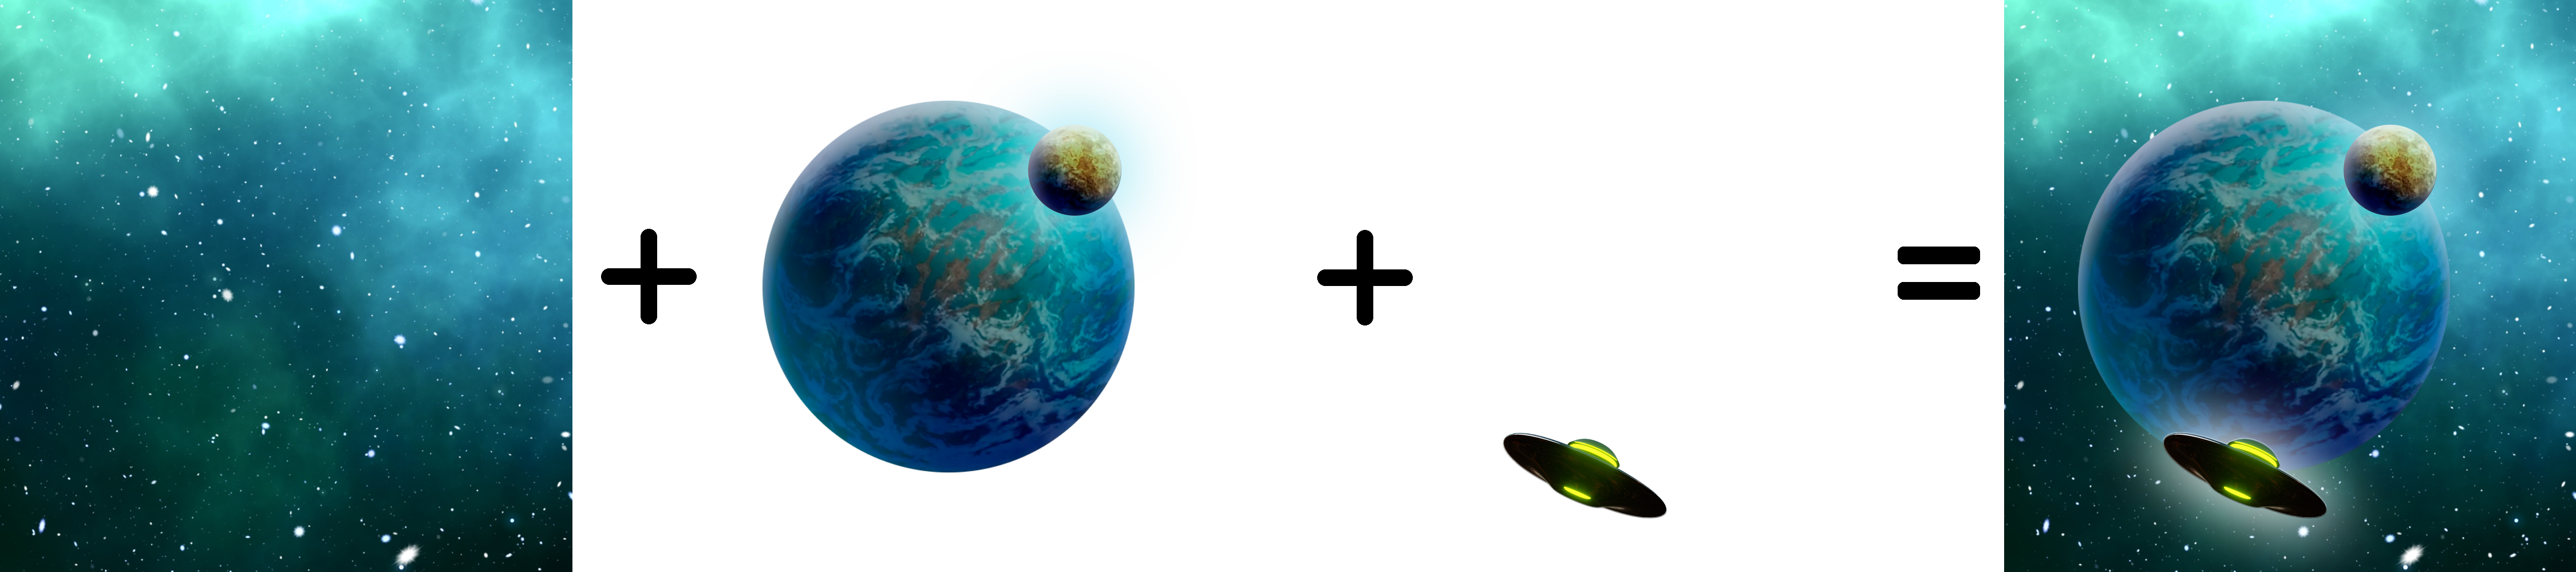
\includegraphics[width=1\textwidth]{images/NFTAutogenerato.png}
    \caption{Esempio di immagine generata}
    \label{fig:esempio-immagine-generata}
\end{figure}


Per quanto riguarda i metadati, questi vengono generati in base alle immagini scelte per ogni \textit{layer}. In seguito alla configurazione del nome e della descrizione della collezione, il file json contenente i metadati relativo alla figura \ref{fig:esempio-immagine-generata} è il seguente:

\begin{lstlisting}[basicstyle=\small]
    {
        "name": "Planet #18",
        "description": "Would you like to live here?",
        "image": "18.png",
        "attributes": [
          {
            "trait_type": "background",
            "value": "lightBlue"
          },
          {
            "trait_type": "planet",
            "value": "blueDouble"
          },
          {
            "trait_type": "flyingObjects",
            "value": "ufo"
          }
        ]
      }
\end{lstlisting}

Nel seguito del progetto è stata riutilizzata la funzionalità di aggiunta automatica dei metadati a IPFS e blockchain. Quindi, l'autogenerazione di immagini non è stata inserita all'interno del marketplace in quanto è spesso compito del creatore fornire i metadati e l'immagine del NFT. Tuttavia, la funzionalità potrebbe essere facilmente aggiunta in futuro.

\subsection{Controllo integrità NFT in vendita}
\label{sec:controllo-integrita-nft-in-vendita}

Nel momento in cui un utente mette in vendita un NFT, il marketplace diventa semplicemente un gestore dell'asset e non il suo possessore. Questo significa che l'utente ha il pieno controllo dell'asset. Infatti, se l'utente decidesse di trasferirlo esternamente al marketplace ad un altro indirizzo, il marketplace non sarebbe in grado di rilevare questo cambiamento e di conseguenza si verificherebbe un errore, come schematizzato in figura \ref{fig:integrita-nft}.


\begin{figure}[H]
    \centering
    \includegraphics[width=1\textwidth]{images/IntegritàNFT.png}
    \caption{Esempio di mancanza di integrità di un vendita}
    \label{fig:integrita-nft}
\end{figure}

Per risolvere tale problema è stato deciso di implementare un controllo di integrità di tutti gli NFT attualmente in vendita. Il microservizio creato analizza tutti i nuovi blocchi generati dalla blockchain, filtrando il contenuto su eventi di tipo \textit{transfer} emessi dai token in vendita. Nel caso in cui esista un evento di questo genere e non sia stato emesso l'evento di vendita dal marketplace, il microservizio invierà una transazione per rimuovere l'asset dalla vendita. In questo modo, il marketplace è sempre in grado di rilevare eventuali cambiamenti di proprietà degli NFT in vendita.